\documentclass{standalone}
\usepackage{tikz}
\usetikzlibrary{patterns, positioning}

\begin{document}
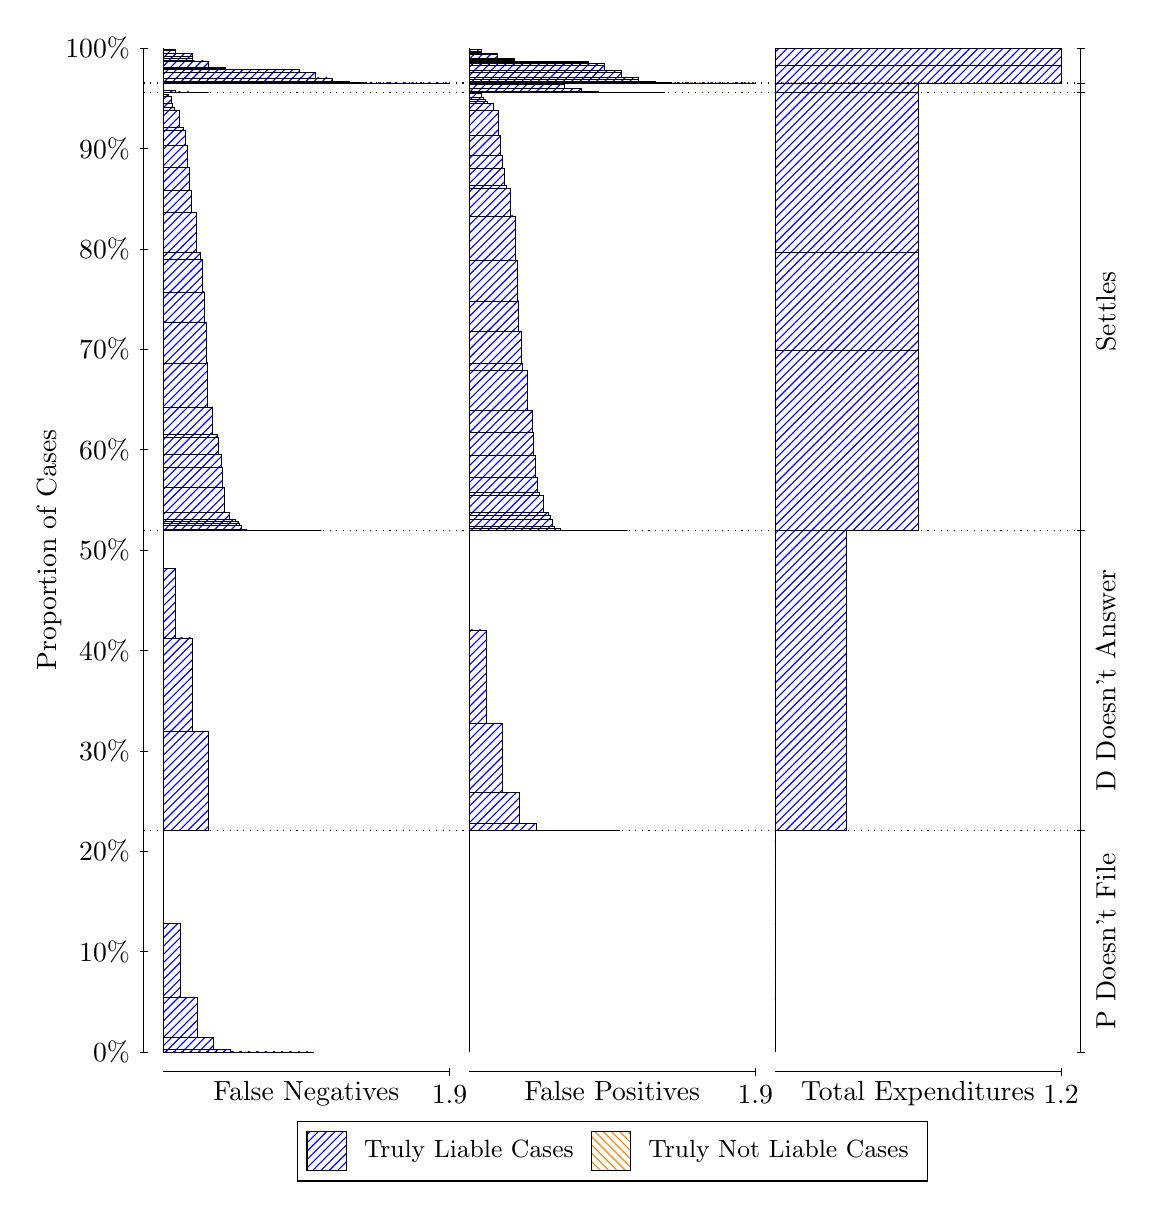
\begin{tikzpicture}
\draw[black, very thin] (1.5,1.75) -- (1.5,14.5);
\node[rotate=90, anchor=center] at (0.3, 8.125) {Proportion of Cases};
\draw[black, very thin] (1.45,1.75) -- (1.55,1.75);
\node[anchor=east] at (1.45, 1.75) {0\%};
\draw[black, very thin] (1.45,3.025) -- (1.55,3.025);
\node[anchor=east] at (1.45, 3.025) {10\%};
\draw[black, very thin] (1.45,4.3) -- (1.55,4.3);
\node[anchor=east] at (1.45, 4.3) {20\%};
\draw[black, very thin] (1.45,5.575) -- (1.55,5.575);
\node[anchor=east] at (1.45, 5.575) {30\%};
\draw[black, very thin] (1.45,6.85) -- (1.55,6.85);
\node[anchor=east] at (1.45, 6.85) {40\%};
\draw[black, very thin] (1.45,8.125) -- (1.55,8.125);
\node[anchor=east] at (1.45, 8.125) {50\%};
\draw[black, very thin] (1.45,9.4) -- (1.55,9.4);
\node[anchor=east] at (1.45, 9.4) {60\%};
\draw[black, very thin] (1.45,10.675) -- (1.55,10.675);
\node[anchor=east] at (1.45, 10.675) {70\%};
\draw[black, very thin] (1.45,11.95) -- (1.55,11.95);
\node[anchor=east] at (1.45, 11.95) {80\%};
\draw[black, very thin] (1.45,13.225) -- (1.55,13.225);
\node[anchor=east] at (1.45, 13.225) {90\%};
\draw[black, very thin] (1.45,14.5) -- (1.55,14.5);
\node[anchor=east] at (1.45, 14.5) {100\%};

\draw[black, very thin] (13.4,1.75) -- (13.4,14.5);
\draw[black, very thin] (13.35,1.75) -- (13.45,1.75);
\node[anchor=west] at (13.35, 1.75) {};
\draw[black, very thin] (13.35,4.5603) -- (13.45,4.5603);
\node[anchor=west] at (13.35, 4.5603) {};
\draw[black, very thin] (13.35,8.3729) -- (13.45,8.3729);
\node[anchor=west] at (13.35, 8.3729) {};
\draw[black, very thin] (13.35,13.94) -- (13.45,13.94);
\node[anchor=west] at (13.35, 13.94) {};
\draw[black, very thin] (13.35,14.056) -- (13.45,14.056);
\node[anchor=west] at (13.35, 14.056) {};
\draw[black, very thin] (13.35,14.5) -- (13.45,14.5);
\node[anchor=west] at (13.35, 14.5) {};

\draw[black, very thin, pattern color=blue, pattern=north east lines] (1.75,1.75) rectangle (3.6623,1.75);
\draw[black, very thin, pattern color=blue, pattern=north east lines] (1.75,1.75) rectangle (3.4498,1.75);
\draw[black, very thin, pattern color=blue, pattern=north east lines] (1.75,1.75) rectangle (3.2373,1.75);
\draw[black, very thin, pattern color=blue, pattern=north east lines] (1.75,1.75) rectangle (3.0249,1.7501);
\draw[black, very thin, pattern color=blue, pattern=north east lines] (1.75,1.7501) rectangle (2.8124,1.7523);
\draw[black, very thin, pattern color=blue, pattern=north east lines] (1.75,1.7523) rectangle (2.5999,1.779);
\draw[black, very thin, pattern color=blue, pattern=north east lines] (1.75,1.779) rectangle (2.3874,1.9392);
\draw[black, very thin, pattern color=blue, pattern=north east lines] (1.75,1.9392) rectangle (2.175,2.4471);
\draw[black, very thin, pattern color=blue, pattern=north east lines] (1.75,2.4471) rectangle (1.9625,3.3812);
\draw[black, very thin, pattern color=orange, pattern=north west lines] (1.75,3.3812) rectangle (1.75,3.3812);
\draw[black, very thin, pattern color=blue, pattern=north east lines] (1.75,3.3812) rectangle (1.75,4.5603);
\draw[black, very thin, pattern color=blue, pattern=north east lines] (1.75,4.5603) rectangle (2.3237,5.8238);
\draw[black, very thin, pattern color=blue, pattern=north east lines] (1.75,5.8238) rectangle (2.1112,7.0076);
\draw[black, very thin, pattern color=blue, pattern=north east lines] (1.75,7.0076) rectangle (1.8987,7.8867);
\draw[black, very thin, pattern color=orange, pattern=north west lines] (1.75,7.8867) rectangle (1.75,7.8867);
\draw[black, very thin, pattern color=blue, pattern=north east lines] (1.75,7.8867) rectangle (1.75,8.3729);
\draw[black, very thin, pattern color=blue, pattern=north east lines] (1.75,8.3729) rectangle (3.7579,8.3729);
\draw[black, very thin, pattern color=blue, pattern=north east lines] (1.75,8.3729) rectangle (3.5667,8.3729);
\draw[black, very thin, pattern color=blue, pattern=north east lines] (1.75,8.3729) rectangle (3.5454,8.3729);
\draw[black, very thin, pattern color=blue, pattern=north east lines] (1.75,8.3729) rectangle (3.3754,8.3729);
\draw[black, very thin, pattern color=blue, pattern=north east lines] (1.75,8.3729) rectangle (3.3542,8.3729);
\draw[black, very thin, pattern color=blue, pattern=north east lines] (1.75,8.3729) rectangle (3.3329,8.3729);
\draw[black, very thin, pattern color=blue, pattern=north east lines] (1.75,8.3729) rectangle (3.2798,8.3729);
\draw[black, very thin, pattern color=blue, pattern=north east lines] (1.75,8.3729) rectangle (3.163,8.373);
\draw[black, very thin, pattern color=blue, pattern=north east lines] (1.75,8.373) rectangle (3.1417,8.373);
\draw[black, very thin, pattern color=blue, pattern=north east lines] (1.75,8.373) rectangle (3.1205,8.373);
\draw[black, very thin, pattern color=blue, pattern=north east lines] (1.75,8.373) rectangle (3.0886,8.373);
\draw[black, very thin, pattern color=blue, pattern=north east lines] (1.75,8.373) rectangle (3.0673,8.373);
\draw[black, very thin, pattern color=blue, pattern=north east lines] (1.75,8.373) rectangle (2.9505,8.3748);
\draw[black, very thin, pattern color=blue, pattern=north east lines] (1.75,8.3748) rectangle (2.9292,8.3758);
\draw[black, very thin, pattern color=blue, pattern=north east lines] (1.75,8.3758) rectangle (2.908,8.3761);
\draw[black, very thin, pattern color=blue, pattern=north east lines] (1.75,8.3761) rectangle (2.8761,8.3767);
\draw[black, very thin, pattern color=blue, pattern=north east lines] (1.75,8.3767) rectangle (2.8549,8.3768);
\draw[black, very thin, pattern color=blue, pattern=north east lines] (1.75,8.3768) rectangle (2.8018,8.3881);
\draw[black, very thin, pattern color=blue, pattern=north east lines] (1.75,8.3881) rectangle (2.738,8.4364);
\draw[black, very thin, pattern color=blue, pattern=north east lines] (1.75,8.4364) rectangle (2.7168,8.4695);
\draw[black, very thin, pattern color=blue, pattern=north east lines] (1.75,8.4695) rectangle (2.6955,8.4865);
\draw[black, very thin, pattern color=blue, pattern=north east lines] (1.75,8.4865) rectangle (2.6636,8.5108);
\draw[black, very thin, pattern color=blue, pattern=north east lines] (1.75,8.5108) rectangle (2.6424,8.5153);
\draw[black, very thin, pattern color=blue, pattern=north east lines] (1.75,8.5153) rectangle (2.5893,8.6036);
\draw[black, very thin, pattern color=blue, pattern=north east lines] (1.75,8.6036) rectangle (2.5255,8.9188);
\draw[black, very thin, pattern color=blue, pattern=north east lines] (1.75,8.9188) rectangle (2.5043,9.1773);
\draw[black, very thin, pattern color=blue, pattern=north east lines] (1.75,9.1773) rectangle (2.483,9.3405);
\draw[black, very thin, pattern color=blue, pattern=north east lines] (1.75,9.3405) rectangle (2.4512,9.5557);
\draw[black, very thin, pattern color=blue, pattern=north east lines] (1.75,9.5557) rectangle (2.4299,9.5997);
\draw[black, very thin, pattern color=blue, pattern=north east lines] (1.75,9.5997) rectangle (2.3768,9.9438);
\draw[black, very thin, pattern color=blue, pattern=north east lines] (1.75,9.9438) rectangle (2.3131,10.502);
\draw[black, very thin, pattern color=blue, pattern=north east lines] (1.75,10.502) rectangle (2.2918,11.023);
\draw[black, very thin, pattern color=blue, pattern=north east lines] (1.75,11.023) rectangle (2.2706,11.404);
\draw[black, very thin, pattern color=blue, pattern=north east lines] (1.75,11.404) rectangle (2.2387,11.822);
\draw[black, very thin, pattern color=blue, pattern=north east lines] (1.75,11.822) rectangle (2.2174,11.911);
\draw[black, very thin, pattern color=blue, pattern=north east lines] (1.75,11.911) rectangle (2.1643,12.411);
\draw[black, very thin, pattern color=blue, pattern=north east lines] (1.75,12.411) rectangle (2.1006,12.689);
\draw[black, very thin, pattern color=blue, pattern=north east lines] (1.75,12.689) rectangle (2.0793,12.986);
\draw[black, very thin, pattern color=blue, pattern=north east lines] (1.75,12.986) rectangle (2.0581,13.265);
\draw[black, very thin, pattern color=blue, pattern=north east lines] (1.75,13.265) rectangle (2.0262,13.457);
\draw[black, very thin, pattern color=blue, pattern=north east lines] (1.75,13.457) rectangle (2.005,13.495);
\draw[black, very thin, pattern color=blue, pattern=north east lines] (1.75,13.495) rectangle (1.9519,13.707);
\draw[black, very thin, pattern color=blue, pattern=north east lines] (1.75,13.707) rectangle (1.8881,13.744);
\draw[black, very thin, pattern color=blue, pattern=north east lines] (1.75,13.744) rectangle (1.8669,13.797);
\draw[black, very thin, pattern color=blue, pattern=north east lines] (1.75,13.797) rectangle (1.8456,13.889);
\draw[black, very thin, pattern color=blue, pattern=north east lines] (1.75,13.889) rectangle (1.8137,13.909);
\draw[black, very thin, pattern color=blue, pattern=north east lines] (1.75,13.909) rectangle (1.7925,13.912);
\draw[black, very thin, pattern color=orange, pattern=north west lines] (1.75,13.912) rectangle (1.75,13.912);
\draw[black, very thin, pattern color=blue, pattern=north east lines] (1.75,13.912) rectangle (1.75,13.94);
\draw[black, very thin, pattern color=blue, pattern=north east lines] (1.75,13.94) rectangle (2.3237,13.94);
\draw[black, very thin, pattern color=blue, pattern=north east lines] (1.75,13.94) rectangle (2.1112,13.942);
\draw[black, very thin, pattern color=blue, pattern=north east lines] (1.75,13.942) rectangle (1.8987,13.96);
\draw[black, very thin, pattern color=orange, pattern=north west lines] (1.75,13.96) rectangle (1.75,13.96);
\draw[black, very thin, pattern color=blue, pattern=north east lines] (1.75,13.96) rectangle (1.75,14.056);
\draw[black, very thin, pattern color=blue, pattern=north east lines] (1.75,14.056) rectangle (5.3833,14.056);
\draw[black, very thin, pattern color=blue, pattern=north east lines] (1.75,14.056) rectangle (5.1709,14.056);
\draw[black, very thin, pattern color=blue, pattern=north east lines] (1.75,14.056) rectangle (4.9584,14.056);
\draw[black, very thin, pattern color=blue, pattern=north east lines] (1.75,14.056) rectangle (4.7459,14.056);
\draw[black, very thin, pattern color=blue, pattern=north east lines] (1.75,14.056) rectangle (4.7459,14.056);
\draw[black, very thin, pattern color=blue, pattern=north east lines] (1.75,14.056) rectangle (4.5334,14.057);
\draw[black, very thin, pattern color=blue, pattern=north east lines] (1.75,14.057) rectangle (4.5334,14.057);
\draw[black, very thin, pattern color=blue, pattern=north east lines] (1.75,14.057) rectangle (4.321,14.057);
\draw[black, very thin, pattern color=blue, pattern=north east lines] (1.75,14.057) rectangle (4.321,14.059);
\draw[black, very thin, pattern color=blue, pattern=north east lines] (1.75,14.059) rectangle (4.1085,14.067);
\draw[black, very thin, pattern color=blue, pattern=north east lines] (1.75,14.067) rectangle (4.1085,14.074);
\draw[black, very thin, pattern color=blue, pattern=north east lines] (1.75,14.074) rectangle (3.896,14.111);
\draw[black, very thin, pattern color=blue, pattern=north east lines] (1.75,14.111) rectangle (3.896,14.121);
\draw[black, very thin, pattern color=blue, pattern=north east lines] (1.75,14.121) rectangle (3.6835,14.192);
\draw[black, very thin, pattern color=blue, pattern=north east lines] (1.75,14.192) rectangle (3.5985,14.192);
\draw[black, very thin, pattern color=blue, pattern=north east lines] (1.75,14.192) rectangle (3.4711,14.224);
\draw[black, very thin, pattern color=blue, pattern=north east lines] (1.75,14.224) rectangle (3.3861,14.224);
\draw[black, very thin, pattern color=blue, pattern=north east lines] (1.75,14.224) rectangle (3.3861,14.224);
\draw[black, very thin, pattern color=blue, pattern=north east lines] (1.75,14.224) rectangle (3.2586,14.224);
\draw[black, very thin, pattern color=blue, pattern=north east lines] (1.75,14.224) rectangle (3.2586,14.228);
\draw[black, very thin, pattern color=blue, pattern=north east lines] (1.75,14.228) rectangle (3.1736,14.228);
\draw[black, very thin, pattern color=blue, pattern=north east lines] (1.75,14.228) rectangle (3.0461,14.228);
\draw[black, very thin, pattern color=blue, pattern=north east lines] (1.75,14.228) rectangle (3.0461,14.228);
\draw[black, very thin, pattern color=blue, pattern=north east lines] (1.75,14.228) rectangle (2.9611,14.228);
\draw[black, very thin, pattern color=blue, pattern=north east lines] (1.75,14.228) rectangle (2.8336,14.228);
\draw[black, very thin, pattern color=blue, pattern=north east lines] (1.75,14.228) rectangle (2.7486,14.228);
\draw[black, very thin, pattern color=blue, pattern=north east lines] (1.75,14.228) rectangle (2.7486,14.229);
\draw[black, very thin, pattern color=blue, pattern=north east lines] (1.75,14.229) rectangle (2.6212,14.229);
\draw[black, very thin, pattern color=blue, pattern=north east lines] (1.75,14.229) rectangle (2.5362,14.229);
\draw[black, very thin, pattern color=blue, pattern=north east lines] (1.75,14.229) rectangle (2.5362,14.232);
\draw[black, very thin, pattern color=blue, pattern=north east lines] (1.75,14.232) rectangle (2.5362,14.241);
\draw[black, very thin, pattern color=blue, pattern=north east lines] (1.75,14.241) rectangle (2.5362,14.253);
\draw[black, very thin, pattern color=blue, pattern=north east lines] (1.75,14.253) rectangle (2.3237,14.253);
\draw[black, very thin, pattern color=blue, pattern=north east lines] (1.75,14.253) rectangle (2.3237,14.338);
\draw[black, very thin, pattern color=blue, pattern=north east lines] (1.75,14.338) rectangle (2.1112,14.34);
\draw[black, very thin, pattern color=blue, pattern=north east lines] (1.75,14.34) rectangle (2.1112,14.367);
\draw[black, very thin, pattern color=blue, pattern=north east lines] (1.75,14.367) rectangle (2.1112,14.396);
\draw[black, very thin, pattern color=blue, pattern=north east lines] (1.75,14.396) rectangle (2.1112,14.43);
\draw[black, very thin, pattern color=blue, pattern=north east lines] (1.75,14.43) rectangle (1.8987,14.437);
\draw[black, very thin, pattern color=blue, pattern=north east lines] (1.75,14.437) rectangle (1.8987,14.469);
\draw[black, very thin, pattern color=blue, pattern=north east lines] (1.75,14.469) rectangle (1.8987,14.48);
\draw[black, very thin, pattern color=orange, pattern=north west lines] (1.75,14.48) rectangle (1.75,14.48);
\draw[black, very thin, pattern color=blue, pattern=north east lines] (1.75,14.48) rectangle (1.75,14.5);
\draw[black, very thin, pattern color=orange, pattern=north west lines] (5.6333,1.75) rectangle (5.6333,1.75);
\draw[black, very thin, pattern color=blue, pattern=north east lines] (5.6333,1.75) rectangle (5.6333,4.5603);
\draw[black, very thin, pattern color=orange, pattern=north west lines] (5.6333,4.5603) rectangle (7.5456,4.5603);
\draw[black, very thin, pattern color=blue, pattern=north east lines] (5.6333,4.5603) rectangle (7.5456,4.5603);
\draw[black, very thin, pattern color=blue, pattern=north east lines] (5.6333,4.5603) rectangle (7.3331,4.5603);
\draw[black, very thin, pattern color=blue, pattern=north east lines] (5.6333,4.5603) rectangle (7.1207,4.5603);
\draw[black, very thin, pattern color=blue, pattern=north east lines] (5.6333,4.5603) rectangle (6.9082,4.5605);
\draw[black, very thin, pattern color=blue, pattern=north east lines] (5.6333,4.5605) rectangle (6.6957,4.5683);
\draw[black, very thin, pattern color=blue, pattern=north east lines] (5.6333,4.5683) rectangle (6.4832,4.6533);
\draw[black, very thin, pattern color=blue, pattern=north east lines] (5.6333,4.6533) rectangle (6.2708,5.0465);
\draw[black, very thin, pattern color=blue, pattern=north east lines] (5.6333,5.0465) rectangle (6.0583,5.9256);
\draw[black, very thin, pattern color=blue, pattern=north east lines] (5.6333,5.9256) rectangle (5.8458,7.1094);
\draw[black, very thin, pattern color=blue, pattern=north east lines] (5.6333,7.1094) rectangle (5.6333,8.3729);
\draw[black, very thin, pattern color=orange, pattern=north west lines] (5.6333,8.3729) rectangle (7.6412,8.3729);
\draw[black, very thin, pattern color=blue, pattern=north east lines] (5.6333,8.3729) rectangle (7.6412,8.3729);
\draw[black, very thin, pattern color=blue, pattern=north east lines] (5.6333,8.3729) rectangle (7.4288,8.3729);
\draw[black, very thin, pattern color=orange, pattern=north west lines] (5.6333,8.3729) rectangle (7.3544,8.3729);
\draw[black, very thin, pattern color=blue, pattern=north east lines] (5.6333,8.3729) rectangle (7.3544,8.3729);
\draw[black, very thin, pattern color=blue, pattern=north east lines] (5.6333,8.3729) rectangle (7.2163,8.3729);
\draw[black, very thin, pattern color=orange, pattern=north west lines] (5.6333,8.3729) rectangle (7.1632,8.3729);
\draw[black, very thin, pattern color=blue, pattern=north east lines] (5.6333,8.3729) rectangle (7.1632,8.3729);
\draw[black, very thin, pattern color=blue, pattern=north east lines] (5.6333,8.3729) rectangle (7.1419,8.373);
\draw[black, very thin, pattern color=orange, pattern=north west lines] (5.6333,8.373) rectangle (7.0675,8.373);
\draw[black, very thin, pattern color=blue, pattern=north east lines] (5.6333,8.373) rectangle (7.0675,8.373);
\draw[black, very thin, pattern color=blue, pattern=north east lines] (5.6333,8.373) rectangle (7.0038,8.3734);
\draw[black, very thin, pattern color=blue, pattern=north east lines] (5.6333,8.3734) rectangle (6.9507,8.3735);
\draw[black, very thin, pattern color=blue, pattern=north east lines] (5.6333,8.3735) rectangle (6.9294,8.3739);
\draw[black, very thin, pattern color=orange, pattern=north west lines] (5.6333,8.3739) rectangle (6.8763,8.3739);
\draw[black, very thin, pattern color=blue, pattern=north east lines] (5.6333,8.3739) rectangle (6.8763,8.3776);
\draw[black, very thin, pattern color=blue, pattern=north east lines] (5.6333,8.3776) rectangle (6.8551,8.379);
\draw[black, very thin, pattern color=blue, pattern=north east lines] (5.6333,8.379) rectangle (6.7913,8.4007);
\draw[black, very thin, pattern color=blue, pattern=north east lines] (5.6333,8.4007) rectangle (6.7382,8.4039);
\draw[black, very thin, pattern color=blue, pattern=north east lines] (5.6333,8.4039) rectangle (6.717,8.4238);
\draw[black, very thin, pattern color=orange, pattern=north west lines] (5.6333,8.4238) rectangle (6.6851,8.4238);
\draw[black, very thin, pattern color=blue, pattern=north east lines] (5.6333,8.4238) rectangle (6.6851,8.5155);
\draw[black, very thin, pattern color=blue, pattern=north east lines] (5.6333,8.5155) rectangle (6.6638,8.5685);
\draw[black, very thin, pattern color=blue, pattern=north east lines] (5.6333,8.5685) rectangle (6.6426,8.6057);
\draw[black, very thin, pattern color=blue, pattern=north east lines] (5.6333,8.6057) rectangle (6.5788,8.8179);
\draw[black, very thin, pattern color=blue, pattern=north east lines] (5.6333,8.8179) rectangle (6.5257,8.8551);
\draw[black, very thin, pattern color=blue, pattern=north east lines] (5.6333,8.8551) rectangle (6.5045,9.047);
\draw[black, very thin, pattern color=blue, pattern=north east lines] (5.6333,9.047) rectangle (6.4726,9.3264);
\draw[black, very thin, pattern color=blue, pattern=north east lines] (5.6333,9.3264) rectangle (6.4514,9.6239);
\draw[black, very thin, pattern color=blue, pattern=north east lines] (5.6333,9.6239) rectangle (6.4301,9.9014);
\draw[black, very thin, pattern color=blue, pattern=north east lines] (5.6333,9.9014) rectangle (6.3664,10.402);
\draw[black, very thin, pattern color=blue, pattern=north east lines] (5.6333,10.402) rectangle (6.3133,10.491);
\draw[black, very thin, pattern color=blue, pattern=north east lines] (5.6333,10.491) rectangle (6.292,10.909);
\draw[black, very thin, pattern color=blue, pattern=north east lines] (5.6333,10.909) rectangle (6.2601,11.289);
\draw[black, very thin, pattern color=blue, pattern=north east lines] (5.6333,11.289) rectangle (6.2389,11.81);
\draw[black, very thin, pattern color=blue, pattern=north east lines] (5.6333,11.81) rectangle (6.2176,12.369);
\draw[black, very thin, pattern color=blue, pattern=north east lines] (5.6333,12.369) rectangle (6.1539,12.713);
\draw[black, very thin, pattern color=blue, pattern=north east lines] (5.6333,12.713) rectangle (6.1008,12.757);
\draw[black, very thin, pattern color=blue, pattern=north east lines] (5.6333,12.757) rectangle (6.0795,12.972);
\draw[black, very thin, pattern color=blue, pattern=north east lines] (5.6333,12.972) rectangle (6.0477,13.135);
\draw[black, very thin, pattern color=blue, pattern=north east lines] (5.6333,13.135) rectangle (6.0264,13.394);
\draw[black, very thin, pattern color=blue, pattern=north east lines] (5.6333,13.394) rectangle (6.0052,13.709);
\draw[black, very thin, pattern color=blue, pattern=north east lines] (5.6333,13.709) rectangle (5.9414,13.797);
\draw[black, very thin, pattern color=blue, pattern=north east lines] (5.6333,13.797) rectangle (5.8883,13.802);
\draw[black, very thin, pattern color=blue, pattern=north east lines] (5.6333,13.802) rectangle (5.8671,13.826);
\draw[black, very thin, pattern color=blue, pattern=north east lines] (5.6333,13.826) rectangle (5.8352,13.843);
\draw[black, very thin, pattern color=blue, pattern=north east lines] (5.6333,13.843) rectangle (5.8139,13.876);
\draw[black, very thin, pattern color=blue, pattern=north east lines] (5.6333,13.876) rectangle (5.7927,13.924);
\draw[black, very thin, pattern color=blue, pattern=north east lines] (5.6333,13.924) rectangle (5.7289,13.936);
\draw[black, very thin, pattern color=blue, pattern=north east lines] (5.6333,13.936) rectangle (5.6758,13.936);
\draw[black, very thin, pattern color=blue, pattern=north east lines] (5.6333,13.936) rectangle (5.6546,13.936);
\draw[black, very thin, pattern color=blue, pattern=north east lines] (5.6333,13.936) rectangle (5.6333,13.94);
\draw[black, very thin, pattern color=orange, pattern=north west lines] (5.6333,13.94) rectangle (8.1193,13.94);
\draw[black, very thin, pattern color=blue, pattern=north east lines] (5.6333,13.94) rectangle (8.1193,13.94);
\draw[black, very thin, pattern color=blue, pattern=north east lines] (5.6333,13.94) rectangle (7.9068,13.94);
\draw[black, very thin, pattern color=blue, pattern=north east lines] (5.6333,13.94) rectangle (7.6943,13.94);
\draw[black, very thin, pattern color=blue, pattern=north east lines] (5.6333,13.94) rectangle (7.4819,13.94);
\draw[black, very thin, pattern color=blue, pattern=north east lines] (5.6333,13.94) rectangle (7.2694,13.945);
\draw[black, very thin, pattern color=blue, pattern=north east lines] (5.6333,13.945) rectangle (7.0569,13.983);
\draw[black, very thin, pattern color=blue, pattern=north east lines] (5.6333,13.983) rectangle (6.8444,14.036);
\draw[black, very thin, pattern color=blue, pattern=north east lines] (5.6333,14.036) rectangle (6.632,14.054);
\draw[black, very thin, pattern color=blue, pattern=north east lines] (5.6333,14.054) rectangle (6.4195,14.056);
\draw[black, very thin, pattern color=blue, pattern=north east lines] (5.6333,14.056) rectangle (6.207,14.056);
\draw[black, very thin, pattern color=orange, pattern=north west lines] (5.6333,14.056) rectangle (9.2667,14.056);
\draw[black, very thin, pattern color=blue, pattern=north east lines] (5.6333,14.056) rectangle (9.2667,14.056);
\draw[black, very thin, pattern color=orange, pattern=north west lines] (5.6333,14.056) rectangle (9.0542,14.056);
\draw[black, very thin, pattern color=blue, pattern=north east lines] (5.6333,14.056) rectangle (9.0542,14.056);
\draw[black, very thin, pattern color=orange, pattern=north west lines] (5.6333,14.056) rectangle (8.8417,14.056);
\draw[black, very thin, pattern color=blue, pattern=north east lines] (5.6333,14.056) rectangle (8.8417,14.056);
\draw[black, very thin, pattern color=blue, pattern=north east lines] (5.6333,14.056) rectangle (8.6292,14.056);
\draw[black, very thin, pattern color=orange, pattern=north west lines] (5.6333,14.056) rectangle (8.6292,14.056);
\draw[black, very thin, pattern color=blue, pattern=north east lines] (5.6333,14.056) rectangle (8.6292,14.056);
\draw[black, very thin, pattern color=orange, pattern=north west lines] (5.6333,14.056) rectangle (8.4168,14.056);
\draw[black, very thin, pattern color=blue, pattern=north east lines] (5.6333,14.056) rectangle (8.4168,14.057);
\draw[black, very thin, pattern color=blue, pattern=north east lines] (5.6333,14.057) rectangle (8.4168,14.057);
\draw[black, very thin, pattern color=orange, pattern=north west lines] (5.6333,14.057) rectangle (8.2043,14.057);
\draw[black, very thin, pattern color=blue, pattern=north east lines] (5.6333,14.057) rectangle (8.2043,14.06);
\draw[black, very thin, pattern color=blue, pattern=north east lines] (5.6333,14.06) rectangle (8.2043,14.06);
\draw[black, very thin, pattern color=blue, pattern=north east lines] (5.6333,14.06) rectangle (7.9918,14.064);
\draw[black, very thin, pattern color=orange, pattern=north west lines] (5.6333,14.064) rectangle (7.9918,14.064);
\draw[black, very thin, pattern color=blue, pattern=north east lines] (5.6333,14.064) rectangle (7.9918,14.077);
\draw[black, very thin, pattern color=blue, pattern=north east lines] (5.6333,14.077) rectangle (7.7793,14.101);
\draw[black, very thin, pattern color=blue, pattern=north east lines] (5.6333,14.101) rectangle (7.7793,14.126);
\draw[black, very thin, pattern color=blue, pattern=north east lines] (5.6333,14.126) rectangle (7.5669,14.191);
\draw[black, very thin, pattern color=blue, pattern=north east lines] (5.6333,14.191) rectangle (7.5669,14.218);
\draw[black, very thin, pattern color=blue, pattern=north east lines] (5.6333,14.218) rectangle (7.3544,14.285);
\draw[black, very thin, pattern color=blue, pattern=north east lines] (5.6333,14.285) rectangle (7.3544,14.303);
\draw[black, very thin, pattern color=blue, pattern=north east lines] (5.6333,14.303) rectangle (7.1419,14.316);
\draw[black, very thin, pattern color=blue, pattern=north east lines] (5.6333,14.316) rectangle (7.1419,14.325);
\draw[black, very thin, pattern color=blue, pattern=north east lines] (5.6333,14.325) rectangle (7.1419,14.327);
\draw[black, very thin, pattern color=orange, pattern=north west lines] (5.6333,14.327) rectangle (7.0569,14.327);
\draw[black, very thin, pattern color=blue, pattern=north east lines] (5.6333,14.327) rectangle (7.0569,14.327);
\draw[black, very thin, pattern color=blue, pattern=north east lines] (5.6333,14.327) rectangle (6.9294,14.328);
\draw[black, very thin, pattern color=blue, pattern=north east lines] (5.6333,14.328) rectangle (6.9294,14.329);
\draw[black, very thin, pattern color=orange, pattern=north west lines] (5.6333,14.329) rectangle (6.8444,14.329);
\draw[black, very thin, pattern color=blue, pattern=north east lines] (5.6333,14.329) rectangle (6.8444,14.329);
\draw[black, very thin, pattern color=blue, pattern=north east lines] (5.6333,14.329) rectangle (6.717,14.329);
\draw[black, very thin, pattern color=blue, pattern=north east lines] (5.6333,14.329) rectangle (6.717,14.329);
\draw[black, very thin, pattern color=blue, pattern=north east lines] (5.6333,14.329) rectangle (6.717,14.329);
\draw[black, very thin, pattern color=blue, pattern=north east lines] (5.6333,14.329) rectangle (6.632,14.329);
\draw[black, very thin, pattern color=orange, pattern=north west lines] (5.6333,14.329) rectangle (6.632,14.329);
\draw[black, very thin, pattern color=blue, pattern=north east lines] (5.6333,14.329) rectangle (6.632,14.329);
\draw[black, very thin, pattern color=blue, pattern=north east lines] (5.6333,14.329) rectangle (6.5045,14.329);
\draw[black, very thin, pattern color=blue, pattern=north east lines] (5.6333,14.329) rectangle (6.5045,14.329);
\draw[black, very thin, pattern color=blue, pattern=north east lines] (5.6333,14.329) rectangle (6.4195,14.33);
\draw[black, very thin, pattern color=orange, pattern=north west lines] (5.6333,14.33) rectangle (6.4195,14.33);
\draw[black, very thin, pattern color=blue, pattern=north east lines] (5.6333,14.33) rectangle (6.4195,14.33);
\draw[black, very thin, pattern color=blue, pattern=north east lines] (5.6333,14.33) rectangle (6.4195,14.332);
\draw[black, very thin, pattern color=blue, pattern=north east lines] (5.6333,14.332) rectangle (6.292,14.332);
\draw[black, very thin, pattern color=blue, pattern=north east lines] (5.6333,14.332) rectangle (6.207,14.347);
\draw[black, very thin, pattern color=orange, pattern=north west lines] (5.6333,14.347) rectangle (6.207,14.347);
\draw[black, very thin, pattern color=blue, pattern=north east lines] (5.6333,14.347) rectangle (6.207,14.351);
\draw[black, very thin, pattern color=blue, pattern=north east lines] (5.6333,14.351) rectangle (6.207,14.364);
\draw[black, very thin, pattern color=blue, pattern=north east lines] (5.6333,14.364) rectangle (6.0795,14.364);
\draw[black, very thin, pattern color=blue, pattern=north east lines] (5.6333,14.364) rectangle (5.9945,14.415);
\draw[black, very thin, pattern color=blue, pattern=north east lines] (5.6333,14.415) rectangle (5.9945,14.435);
\draw[black, very thin, pattern color=blue, pattern=north east lines] (5.6333,14.435) rectangle (5.7821,14.442);
\draw[black, very thin, pattern color=blue, pattern=north east lines] (5.6333,14.442) rectangle (5.7821,14.458);
\draw[black, very thin, pattern color=blue, pattern=north east lines] (5.6333,14.458) rectangle (5.7821,14.482);
\draw[black, very thin, pattern color=blue, pattern=north east lines] (5.6333,14.482) rectangle (5.6333,14.5);
\draw[black, very thin, pattern color=orange, pattern=north west lines] (9.5167,1.75) rectangle (9.5167,1.75);
\draw[black, very thin, pattern color=blue, pattern=north east lines] (9.5167,1.75) rectangle (9.5167,4.5603);
\draw[black, very thin, pattern color=orange, pattern=north west lines] (9.5167,4.5603) rectangle (10.425,4.5603);
\draw[black, very thin, pattern color=blue, pattern=north east lines] (9.5167,4.5603) rectangle (10.425,8.3729);
\draw[black, very thin, pattern color=orange, pattern=north west lines] (9.5167,8.3729) rectangle (11.333,8.3729);
\draw[black, very thin, pattern color=blue, pattern=north east lines] (9.5167,8.3729) rectangle (11.333,10.662);
\draw[black, very thin, pattern color=orange, pattern=north west lines] (9.5167,10.662) rectangle (11.333,10.662);
\draw[black, very thin, pattern color=blue, pattern=north east lines] (9.5167,10.662) rectangle (11.333,11.902);
\draw[black, very thin, pattern color=orange, pattern=north west lines] (9.5167,11.902) rectangle (11.333,11.902);
\draw[black, very thin, pattern color=blue, pattern=north east lines] (9.5167,11.902) rectangle (11.333,13.94);
\draw[black, very thin, pattern color=orange, pattern=north west lines] (9.5167,13.94) rectangle (11.333,13.94);
\draw[black, very thin, pattern color=blue, pattern=north east lines] (9.5167,13.94) rectangle (11.333,14.056);
\draw[black, very thin, pattern color=orange, pattern=north west lines] (9.5167,14.056) rectangle (13.15,14.056);
\draw[black, very thin, pattern color=blue, pattern=north east lines] (9.5167,14.056) rectangle (13.15,14.283);
\draw[black, very thin, pattern color=orange, pattern=north west lines] (9.5167,14.283) rectangle (13.15,14.283);
\draw[black, very thin, pattern color=blue, pattern=north east lines] (9.5167,14.283) rectangle (13.15,14.5);
\draw[black, dotted] (1.5,4.5603) -- (13.4,4.5603);
\draw[black, dotted] (1.5,8.3729) -- (13.4,8.3729);
\draw[black, dotted] (1.5,13.94) -- (13.4,13.94);
\draw[black, dotted] (1.5,14.056) -- (13.4,14.056);
\draw[black, very thin] (1.75,1.5) -- (5.3833,1.5);
\node[anchor=north] at (3.5667, 1.5) {False Negatives};
\draw[black, very thin] (5.3833,1.45) -- (5.3833,1.55);
\node[anchor=north] at (5.3833, 1.45) {1.9};

\draw[black, very thin] (5.6333,1.5) -- (9.2667,1.5);
\node[anchor=north] at (7.45, 1.5) {False Positives};
\draw[black, very thin] (9.2667,1.45) -- (9.2667,1.55);
\node[anchor=north] at (9.2667, 1.45) {1.9};

\draw[black, very thin] (9.5167,1.5) -- (13.15,1.5);
\node[anchor=north] at (11.333, 1.5) {Total Expenditures};
\draw[black, very thin] (13.15,1.45) -- (13.15,1.55);
\node[anchor=north] at (13.15, 1.45) {1.2};

\node[black, centered, rotate=90] at (13.72, 3.1551) {P Doesn't File};
\node[black, centered, rotate=90] at (13.72, 6.4666) {D Doesn't Answer};
\node[black, centered, rotate=90] at (13.72, 11.156) {Settles};



\draw (7.449999999999999,1.5) node[draw=none] (baseCoordinate) {};
\begin{scope}[align=center]
        \matrix[scale=0.5, draw=black, below=0.5cm of baseCoordinate, nodes={draw}, column sep=0.1cm]{
            \node[rectangle, draw, minimum width=0.5cm, minimum height=0.5cm, pattern=north east lines, pattern color=blue] {}; &
            \node[draw=none, font=\small] (B) {Truly Liable Cases}; &
            \node[rectangle, draw, minimum width=0.5cm, minimum height=0.5cm, pattern=north west lines, pattern color=orange] {}; &
            \node[draw=none, font=\small] (B) {Truly Not Liable Cases}; \\
            };
\end{scope}

\end{tikzpicture}
\end{document}